\documentclass[]{article}
\usepackage[margin=1.25in]{geometry}
\usepackage{amsmath,amsthm}
\usepackage{graphicx,tikz}

%opening
\title{Residue Theorem}
\author{Vincent La}

\begin{document}

\maketitle

\begin{abstract}

\end{abstract}

\section{Definitions}
\paragraph{Simple, Closed Contour}
A simple closed contour is:
\begin{itemize}
	\item A contour: An arc consisting of a finite union of smooth curves, connected end to end
	\item Simple: A curve that doesn't intersect itself
	\item Closed: Has the same starting and end point--i.e. it has no opening
	\item Examples: A circle, or the boundary of a square or triangle in a certain direction
\end{itemize}

\begin{center}
	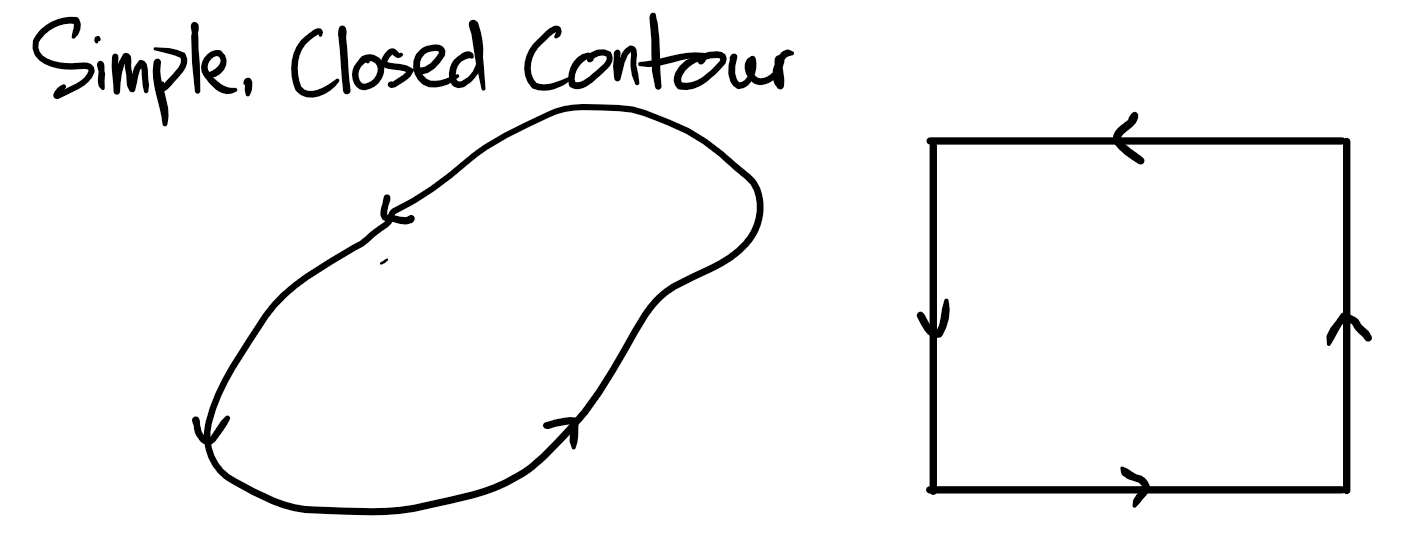
\includegraphics[width=4in]{SimpleClosedContour.png}
\end{center}

\section{Proof}
\subsection{Cauchy-Goursat Theorem}
\subsection{Residues}
\subsection{Residue Theorem}

\section{Example}
\textbf{Source:} Complex Variables and Applications, pg. 159

Use the theorem to evaluate the integral
\[\int_C \frac{5z - 2}{z(z-1)} dz \]
where $C$ is the circle $|z| = 2$ described counterclockwise.

\paragraph{Does It Apply}
\begin{itemize}
	\item A circle is clearly a simple closed contour
	\item $f(z)$ can be written in terms of $z$, so it is analytic except for where we are dividing by zero
\end{itemize}

\paragraph{Singular Points}
This function has two isolated singularities at $z = 0$ and $z = 1$.

\subsection{Solution}
We're going to evaluate this integral by finding the two residues corresponding to our singular points.

\paragraph{First Residue}
First, recall the MacLaurin series
\[\frac{1}{1-z} = \sum^{\infty}_{n=0} z^n = 1 + z + z^2 + ...\]
which is valid for $|z| < 1$.

This allows us to write the Laurent expansion as
\[\begin{aligned}
\frac{5z - 2}{z(z-1)}
&= \frac{5z - 2}{z} \cdot (\frac{-1}{-1})(\frac{1}{z-1}) \\
&= \frac{5z - 2}{z} \cdot \frac{-1}{1 - z} \\
&= \frac{5z - 2}{z} \cdot -\sum^{\infty}_{n=0} z^n & \text{Using MacLaurin series} \\
&= (5 - \frac{2}{z}) \cdot (-1 - z - z^2 - ...)
\end{aligned}\]

Now, because we're only interested in the $b_1$ term, I'm only going to foil the left-side quantity with the first three terms of the right-side quantity. By inspection, there will be no terms in the form $\frac{b_1}{z - z_0}$ once we foil past the first three RHS terms, so we can safely ignore the rest.

Expanding the terms as explained above, we get
\[\begin{aligned}
\frac{5z - 2}{z(z-1)}
&= (5 - \frac{2}{z}) \cdot (-1 - z - z^2 - ...) \\
&= -5 + 5z + \frac{2}{z} + \frac{2z}{z} + 5z^2 \\
&= (-5 + 2) + (5 - 2)z + \frac{2}{z} + ... \\
&= -\frac{2}{z} - 3 - 3z \\
\end{aligned}\]

This implies that $b_1 = -3$.

\paragraph{Second Residue} We can't directly use the same MacLaurin series above because it's not valid at $z = 1$, so we'll perform the change of variables $z = z - 1$.

Thus, we get
\[\begin{aligned}
\frac{5z - 2}{z(z-1)}
&= \frac{5z - 2}{z} \cdot \frac{-1}{1-z} &\text{Same as earlier}\\
&= \frac{5(z-1) - 2}{z-1} \cdot \frac{-1}{1 - (z-1)} &\text{Applying the change of variables}\\
\end{aligned}\]

which is valid for $0 < |z - 1| < 1$.

\end{document}
